\documentclass[aspectratio=1610]{beamer}
\usetheme{boxes}
\usecolortheme{crane}
\usepackage{amsmath,amsfonts}
\usepackage{algpseudocode}
\usepackage{multicol}
\usepackage{pgfplots}
\pgfplotsset{compat=1.15}
\usepackage{mathrsfs}
\usetikzlibrary{arrows}


%-------------------------------------------------------------------
%	 TITLE SLIDE
%-------------------------------------------------------------------


\begin{document}

% -------------------------------------------------------------------
% Lesson 2
% -------------------------------------------------------------------
\section{Software specifications. Formal methods}

\begin{frame}
\begin{center}
\Huge Lesson 2\\~\\
\textbf{Software specifications. Formal methods}
\end{center}
\end{frame}


\begin{frame}
\frametitle{Lesson 2}

\Huge In this lesson we will talk about:
 \alert{Software specifications},
 \alert{Formal methods},
 \alert{Software verification and validation}
\end{frame}



\begin{frame}
\begin{center}
\Huge
\begin{quote}
\textbf{"Todays software has grown by evolution, not by intelligent design"}
\begin{flushright}
{--- Leslie Lamport}	
\end{flushright}
\end{quote}
\end{center}
\end{frame}


\begin{frame}{Lesson 2}{}
\includegraphics[scale=0.30]{Images/loc.png}
\end{frame}


\begin{frame}{Lesson 2}{}
\Huge
 Our software is getting more and more \textbf{complex}, \textbf{buggy} and \textbf{difficult} to maintain.
 \end{frame}


\begin{frame}[plain,noframenumbering]
\makebox[\linewidth]{\includegraphics[width=\paperwidth]{Images/outage1}}
\end{frame}

\begin{frame}[plain,noframenumbering]
\makebox[\linewidth]{\includegraphics[width=\paperwidth]{Images/outage2}}
\end{frame}

\begin{frame}[plain,noframenumbering]
\makebox[\linewidth]{\includegraphics[width=\paperwidth]{Images/outage3}}
\end{frame}

\begin{frame}{Lesson 2}{}
\Huge
\center
    \textbf{What can we do about it?} 
\end{frame}



\begin{frame}{Lesson 2}{}
\Huge
\center
   Start with a \textbf{smart design} at the specification level
\end{frame}


\begin{frame}{Lesson 2}{}
\begin{center}
\Huge\textbf{Software Specifications}
\end{center}
\end{frame}


\begin{frame}{Lesson 2}{}
\Huge{What is a computer specification?}
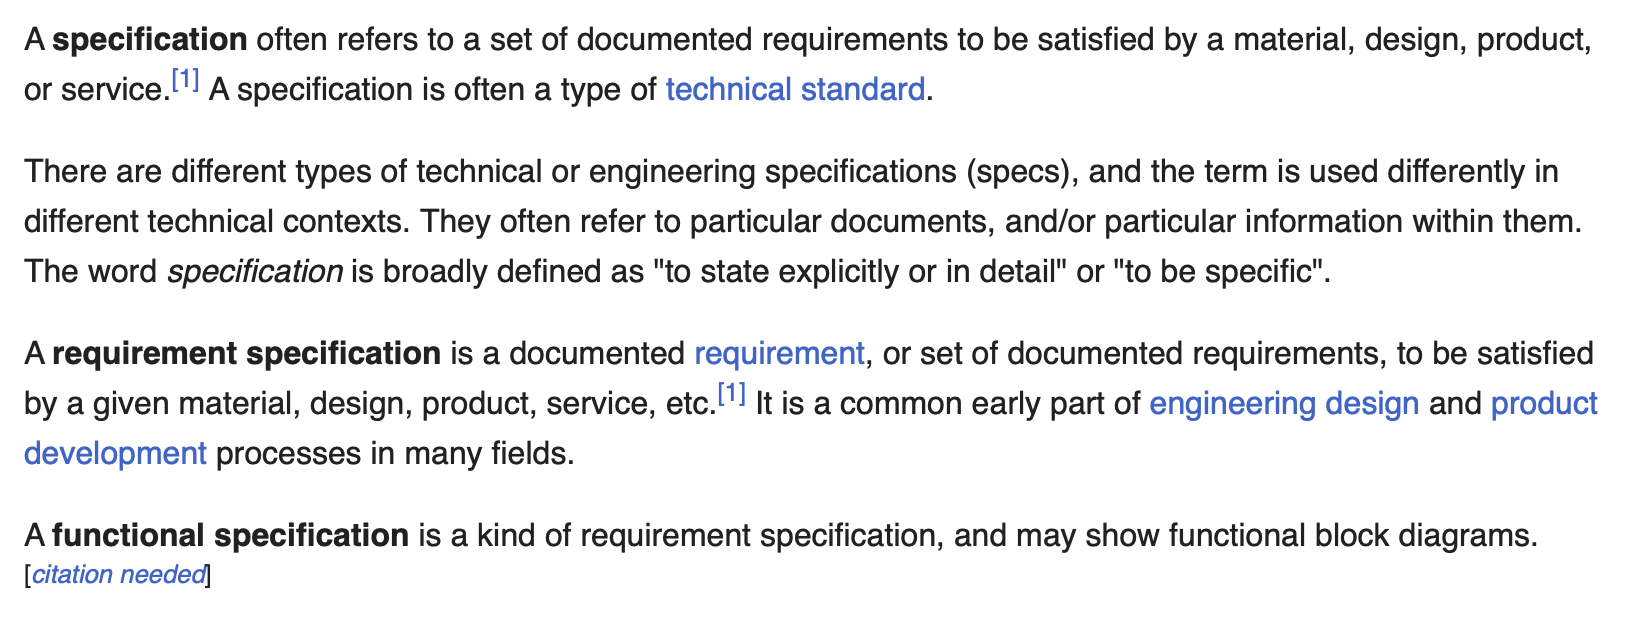
\includegraphics[scale=0.52]{Images/specs}
\end{frame}


\begin{frame}{Lesson 2}{}
\Huge{What is a software specification?}
\includegraphics[scale=0.52]{Images/sfwspecs}
\end{frame}


\begin{frame}{Lesson 2}{}
\Huge
    A \textbf{Software Specification} is a 
    \alert{written} description of what a our application or program 
    is supposed to do.
\end{frame}




\begin{frame}{Lesson 2}{}
\Huge
    A \textbf{Software Specification} is a
    \alert{written} description of what a our application or program
    is supposed to do.
\end{frame}


\begin{frame}{Lesson 2}{}
\Huge
    We call these \alert{\textbf{functional}} specifications 
\end{frame}

%
%https://www.geeksforgeeks.org/functional-vs-non-functional-requirements/

\begin{frame}{Lesson 2}{}
\includegraphics[scale=0.30]{Images/fvsnf.png}
\end{frame}




\begin{frame}{Lesson 2}{}
\LARGE
\textbf{Functional specifications}\\~\\
help us understand our software or application. It’s a very good idea to understand a
system before building it, and that means to write a specification of our program
\alert{before} implementing it.
\end{frame}



%%% Examples of specifications
\begin{frame}{Lesson 1}{}
\Large
\textbf{Examples of specifications}\\~\\
Here are few examples of software soecifications
time.\\~\\
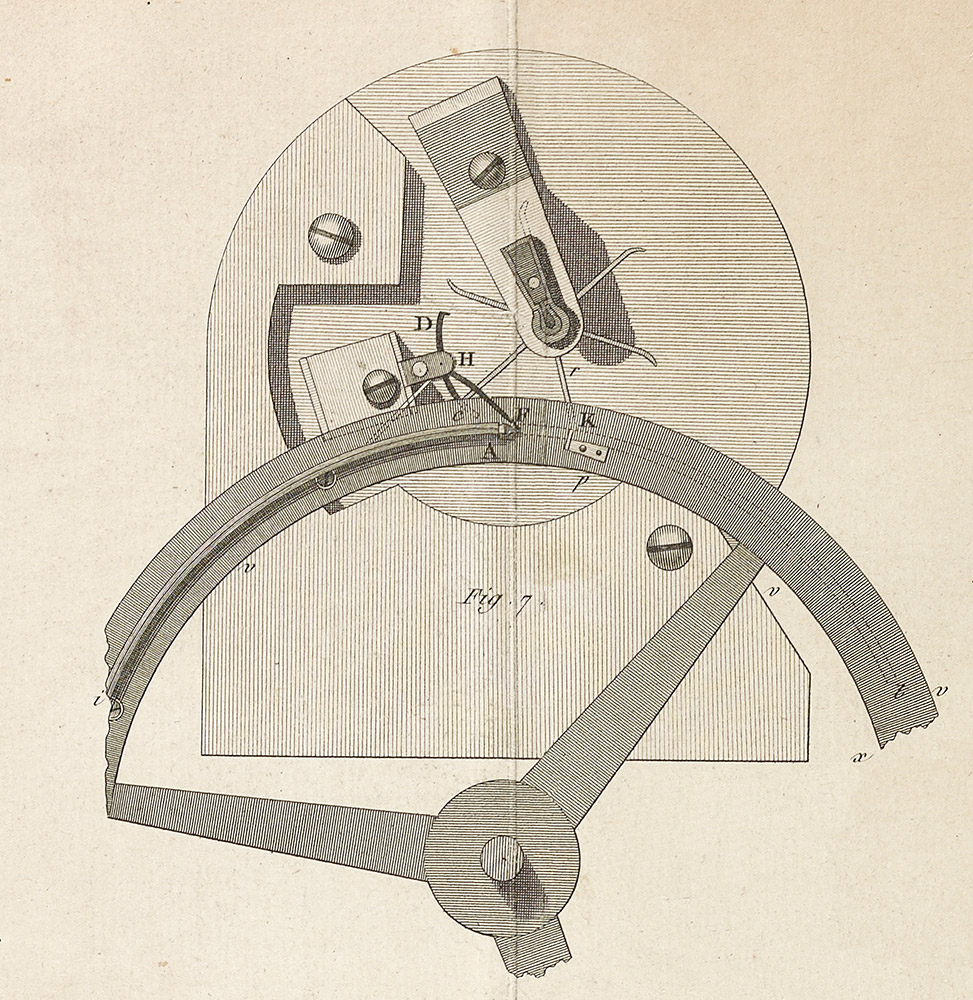
\includegraphics[scale=0.15]{Images/Le_Roy_escapement_mechanism}
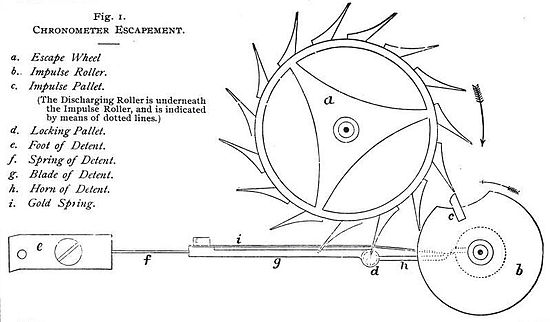
\includegraphics[scale=0.25]{Images/chronometer_detent_escapement}
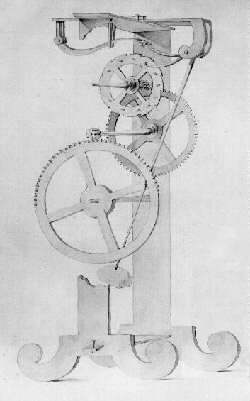
\includegraphics[scale=0.35]{Images/Galileo_Pendulum_Clock}
\end{frame}



\begin{frame}{Lesson 2}{}
\LARGE
\textbf{How can we write the specification?}\\~\\
\begin{itemize}
    \item English. Finnish. Chinese
    \item Graphical diagrams. Drawing
    \item Technical sketches. Mockups
\end{itemize}

\Large
\textbf But all these are imprecise. How can we be precise? What does it mean to be precise?
\end{frame}



\begin{frame}{Lesson 2}{}
\Huge
    A \textbf{The specification is the program} is a
    \alert{written} description of what a our application or program
    is supposed to do.
\end{frame}












\begin{frame}{Lesson 2}{}
\Huge
	Imprecision can lead to \alert{\textbf{ERRORS!}}
\end{frame}


\begin{frame}{Lesson 2}{}
\LARGE
\textbf{Precise specifications}\\~\\
Its difficult to be precise using English or Chinese. Thats why in science and 
engineering fields precise specifications have adopted basic maths to describe 
the specifications.
\end{frame}


\begin{frame}{Lesson 2}{}
\LARGE
\textbf{Basic maths?}\\~\\
Ordinary math. Elementary mathematics. Propositional logic.
\end{frame}

<<<<<<< HEAD
=======

\begin{frame}{Lesson 2}{}
\LARGE
\textbf{Precise Specifications}\\~\\
% image insert
\end{frame}




\begin{frame}{Lesson 2}{}
\LARGE
\textbf{}\\~\\
A computer
system differs from the systems traditionally studied by scientists because we can
pretend that its state changes in discrete steps. So, we represent the execution
of a system as a sequence of states. Formally, we define a behavior to be a
sequence of states, where a state is an assignment of values to variables. We
specify a system by specifying a set of possible behaviors—the ones representing
a correct execution of the system


>>>>>>> 896c40fe12139ccf0e9e8175882ace19dca0fc20
\end{document}

